%%%%%%%%%%%%%%%%%%%%%%%%%%%%%%%%%%%%%%%%%%%%%%%%%%%%%%%%%%%%
%%% LIVECOMS ARTICLE TEMPLATE FOR BEST PRACTICES GUIDE
%%% ADAPTED FROM ELIFE ARTICLE TEMPLATE (8/10/2017)
%%%%%%%%%%%%%%%%%%%%%%%%%%%%%%%%%%%%%%%%%%%%%%%%%%%%%%%%%%%%
%%% PREAMBLE
\documentclass[9pt,tutorial]{livecoms}
% Use the 'onehalfspacing' option for 1.5 line spacing
% Use the 'doublespacing' option for 2.0 line spacing
% Use the 'lineno' option for adding line numbers.
% Use the "ASAPversion' option following article acceptance to add the DOI and relevant dates to the document footer.
% Use the 'pubversion' option for adding the citation and publication information to the document footer, when the LiveCoMS issue is finalized.
% The 'bestpractices' option for indicates that this is a best practices guide.
% Omit the bestpractices option to remove the marking as a LiveCoMS paper.
% Please note that these options may affect formatting.

\usepackage{lipsum} % Required to insert dummy text
\usepackage[version=4]{mhchem}
\usepackage{siunitx}

\usepackage{listings}
\definecolor{mygreen}{rgb}{0,0.5,0}
\lstset{
	basicstyle=\small\ttfamily,
	breakatwhitespace=true,
	breaklines=true,
	language=Python,
	stringstyle=\color{mygreen},
	keywordstyle=\color{blue},
	keywordstyle={[2]\color{blue}}, 
	identifierstyle=\color{black},
	showspaces=false, 
	showstringspaces=false,
	frame=L,
	xleftmargin=\parindent,
	deletekeywords=[2]{type,bin}
}


\DeclareSIUnit\Molar{M}
\usepackage[italic]{mathastext}
\graphicspath{{figures/}}

%%%%%%%%%%%%%%%%%%%%%%%%%%%%%%%%%%%%%%%%%%%%%%%%%%%%%%%%%%%%
%%% IMPORTANT USER CONFIGURATION
%%%%%%%%%%%%%%%%%%%%%%%%%%%%%%%%%%%%%%%%%%%%%%%%%%%%%%%%%%%%
% you should update the minor version number in preprints and major version number of submissions.
\newcommand{\versionnumber}{1.0}

%this should be the main github repository for this article
\newcommand{\githubrepository}{\url{https://github.com/AlleksD/pysimm_lcms_guide}}  

%%%%%%%%%%%%%%%%%%%%%%%%%%%%%%%%%%%%%%%%%%%%%%%%%%%%%%%%%%%%
%%% ARTICLE SETUP
%%%%%%%%%%%%%%%%%%%%%%%%%%%%%%%%%%%%%%%%%%%%%%%%%%%%%%%%%%%%
\title{Introduction to \textit{in silico} synthesis of polymers via PySIMM [Article v\versionnumber]}

\author[1,2,3*]{Alexander G. Demidov}
\author[1,2,3]{B. Lakshitha A. Perera}
\author[1,2,3]{Michael E. Fortunato}
\author[4]{Sibo Lin}
\author[1,2,3,5*]{Coray M. Colina}

\affil[1]{Department of Chemistry, University of Florida, Gainesville, FL 32611, USA}
\affil[2]{George and Josephine Butler Polymer Research Laboratory, University of Florida, Gainesville, FL 32611, USA}
\affil[3]{Center for Macromolecular Science and  Engineering, University of Florida, Gainesville, FL 32611, USA}
\affil[4]{Aramco Services Company: Aramco Research Center - Boston, 400 Technology Square, Cambridge, MA, 02139, USA}
\affil[5]{Department of Materials Science and Engineering, University of Florida, Gainesville, FL 32611 }

\corr{alleks.g.d@ufl.edu}{AD}  % Correspondence emails; appropriate authors initials.
\corr{colina@chem.ufl.edu}{CMC}


\orcid{B. Lakshitha A. Perera}{0000-0003-3015-3529}
\orcid{Coray M. Colina}{0000-0003-2367-1352}

% \contrib[\authfn{1}]{These authors contributed equally to this work}
% \contrib[\authfn{2}]{These authors also contributed equally to this work}

% \presentadd[\authfn{3}]{Department, Institute, Country}
% \presentadd[\authfn{4}]{Department, Institute, Country}

\blurb{This LiveCoMS document is maintained online on GitHub at \githubrepository; to provide feedback, suggestions, or help improve it, please visit the GitHub repository and participate via the issue tracker.}


%%%%%%%%%%%%%%%%%%%%%%%%%%%%%%%%%%%%%%%%%%%%%%%%%%%%%%%%%%%%
%%% PUBLICATION INFORMATION
%%% Fill out these parameters when available
%%% These are used when the "pubversion" option is invoked
%%%%%%%%%%%%%%%%%%%%%%%%%%%%%%%%%%%%%%%%%%%%%%%%%%%%%%%%%%%%
\pubDOI{10.XXXX/YYYYYYY}
\pubvolume{<volume>}
\pubissue{<issue>}
\pubyear{<year>}
\articlenum{<number>}
\datereceived{Day Month Year}
\dateaccepted{Day Month Year}


%%%%%%%%%%%%%%%%%%%%%%%%%%%%%%%%%%%%%%%%%%%%%%%%%%%%%%%%%%%%
%%% ARTICLE START
%%%%%%%%%%%%%%%%%%%%%%%%%%%%%%%%%%%%%%%%%%%%%%%%%%%%%%%%%%%%

\begin{document}

\begin{frontmatter}
\maketitle

\begin{abstract}
Pysimm is a framework for molecular simulations of polymers and polymer-based nanostructures, which enables their direct chemical synthesis and preparation. Pysimm facilitates the understanding of novel, amorphous, processable materials for a broad range of applications, including heterogeneous catalysts, adsorbents and gas storage materials, as well as protein-polymer conjugates. This tutorial provides a detailed guide on the construction of atomistic and united-atom models of polymers using Pysimm: an open-source Python Application Programming Interface for atomistic molecular simulations. The API complements and simplifies the work of widely known molecular simulation software, such as LAMMPS, CASSANDRA, NAMD and Amber. Readers should be familiar with the basic concepts of atomistic molecular simulations, as well as the basic knowledge of Python programming language, before attempting to follow this tutorial.  This work is separated into 3 main sections. First, the process of building an atomic-level model of a polymer chain from its repetitive units is described.  The second section shows how to work with existing forcefields, and how Pysimm can automatically read, recognize, and assign appropriate Force Field parameters to a molecule. The final section discusses how to use Pysimm to construct polymer chains with pre-specified tacticity. The section is also available in the form of an interactive Jupyter notebook tutorial outlining simple guidelines to construct polymer models.

\end{abstract}

\end{frontmatter}


\section{Introduction}

Molecular dynamics (MD) simulations have traditionally been used to study the dynamics of a broad set of systems, from native protein structures, to polymeric materials, at both the all-atom and coarse-grain level of detail \cite{Frenkel_1996, Leach_2001}. Recent advances in this area have expanded into studying protein-polymer hybrids in systems where polymers were either covalently or non-covalently attached \cite{bioconjug_nextgen}. Demystifying protein-polymer interactions, dynamic changes over time, and subtle initiator- or polymer-induced changes to protein structure through MD is central to these goals \cite{Lin2019, lak_2021}. Therefore, integrated platforms need to be developed that can in part retain the detailed resolution of atomistic simulations while expanding the accessible time and length scales required for thorough and efficient study of molecular chimeras.
Although many force fields (FFs) in the biomolecular and small molecule community are optimized using specific water models to reproduce properties under conditions of interest, some water models clearly perform better in representing the general properties of water than others. Moreover, for polymer-water systems, choosing the correct FF for polymers is often ambiguous, and thorough validation with experimental data is often needed \cite{kubota-kubota, kubota-kubota2, tacx2000, bucholz2017, Rukmani2019}.  For example, recent work has led to the trustworthiness (through development and validation) of appropriate FFs for PEGylated proteins at the atomistic- and meso-level scales \cite{farhad_2018, aravinda_peg1}. A major limitation in the development of molecular simulation models for water-soluble polymers and protein-polymer conjugates is the lack of FFs for non-PEG-like water-soluble polymers of interest, as well as the lack of experimental data to validate such FFs. To approach the study of these complex polymeric materials from an atomistic molecular simulation standpoint, it is essential that the FFs used are able to accurately capture the critical polymer-water interactions, as well as the tacticity of such polymer chains.  This in turn necessitates a detailed FF analysis, for both polymer and water, to validate that the models implemented are sampling the appropriate conformational space prior to being utilized to aid in the design of new polymeric materials and protein/polymer complex systems. 

To enable the simulations, we developed, and made available to the broader community, a \textbf{Py}thon based \textbf{S}imulation \textbf{I}nterface for \textbf{M}olecular \textbf{M}odeling, PySIMM. The interface is an open source Python package designed to assist in the setup and execution of molecular simulations through a high-level application program interface (API) and abstraction from underlying third-party simulation software. So far it includes the ability to perform molecular dynamic simulations (using the LAMMPS engine\cite{lammps}), Monte Carlo simulations (using the CASSANDRA software \cite{cassandra}), and a few types of fractional free volume analyses (provided by Poreblazer \cite{pblazer} and/or Zeo++ \cite{zeopp} software). Pysimm has been used for several studies involving simulation of atomic-scale polymer models \cite{Rukmani2019_pegda, song2020, anstine2020effects} and recently it was expanded \cite{pysimm_upd2} to build polymer models convenient for bioconjugates modeling as described in this tutorial. 

\subsection{Scope}

This tutorial is separated into 3 parts and will walk the reader through the entire process of building an atomic-level model of a polymer chain (or a polymer melt) from scratch. The first part is concentrated on the basics of pysimm that allow the reader to build a 'small' molecule as a repetitive unit that can be later used in the construction of a macromolecule. In this, we introduce basic pysimm abstractions and list the ways in which a molecule can be imported to pysimm representation. 
The second part discusses the work with force field parameters and the extent to which pysimm can automatically read, recognize, and assign appropriate FF parameters to a molecule. We will use an example simulation setup to illustrate how to apply/switch a FF for a molecular system using  GAFF, and the CHARMM general force field (CGenFF). Finally, the third part discusses the utilization of the force field assisted random walk application, and its modifications to build a macromolecule. In this part, we specifically focus on the tacticity properties of the constructed polymer chains. 

The present work is designed to give the readers a relatively simple, yet versatile instrument to build their own atomic-scale models of polymers with precise control over the chain length (or polydispersity index), monomer sequence in copolymers, and polymer chain tacticity. 


% <--------------------------------------------------------------------
% <----------------------Tutorial Prerequisites------------------------
% <--------------------------------------------------------------------
\section{Prerequisites}

\subsection{Background knowledge}

The tutorial aims to describe the basic concepts for working with the API for molecular modeling. Correspondingly, readers are expected to be familiar with the basic concepts of atomistic molecular simulations such as (i) functional forms of common class-I FFs and their representation of van der Waals and electrostatic interactions; (ii) basic information about the way the MD equations are integrated, i.e. the most appropriate integration schemes, optimal time step and other possible integration settings; (iii) additional positional constraints that are often imposed on a molecular system (e.g. application of the SHAKE algorithm for the simulation of water models).

\subsection{Software/system requirements}

As readers will work with a Python-based API, the basic knowledge of Python programming language such as: (i) constructors of basic dynamic data structures (lists, sets, and dictionaries), (ii) functions and their arguments, (iii) strings and basic file input/output is required. 
The main tool that provides the means for molecular simulations is LAMMPS. Thus the next section briefly discusses how to obtain the pysimm code, and integrate it with LAMMPS (either existing or freshly installed). Please note that all instructions are fit for Linux distributions (Ubuntu, OpenSUSE, and CentOS distributions had been tested) and had not been tested on Windows. However, tools like Cygwin and other Linux environment emulators likely can cover the functionality that is necessary to run pysimm with LAMMPS on Windows. 

\subsubsection{Docker image with pysimm deployed}

One convenient way to use pysimm is the work with the Docker image.
The image already contains pysimm and all necessary software dependencies to run this tutorial, so if you choose to work with the image there is no need to install pysimm to your OS, as it is described below in this section.

The \textit{Dockerfile.txt} instructions to build the corresponding image are in the root folder of pysimm distribution. The routine for building and usage the Docker image is standard. To build the Docker image from the file, run the following from the root pysimm directory (optionally changing \lstinline$my_tag$ to any meaningful text tag of your image):

\begin{lstlisting}
$ docker build -t pysimm:my_tag -f Dockerfile $PWD
\end{lstlisting}

This will create a Docker image based on the Debian 10 Linux distribution with pysimm and pre-installed LAMMPS, CASSANDRA, Zeo++ v0.3, and PoreBlazer v4.0. If the build is successful the list of your Docker images will contain freshly built pysimm image. The full list can be seen by running \lstinline$docker images$ command. 

After the successful build, run the corresponding pysimm image in bash mode:
\begin{lstlisting}
$ docker run -it pysimm:my_tag bash
\end{lstlisting}

The pysimm source files are kept in \lstinline$/usr/local/pysimm$ folder. Thus one can quickly test the LAMMPS or CASSANDRA modules by running one of the examples, for instance:

\begin{lstlisting}
$ cd /usr/local/pysimm
$ cd Examples/08_ethanol_acetone_mixture
$ python run.py
\end{lstlisting}

The successful run of the example will create input text files called 'mixture.*' which contain the simulated equilibrated ethanol/acetone mixture.


\subsubsection{Native pysimm installation}

This subsection describes how to install pysimm on your operating system directly. To get started, clone the pysimm repository from GitHub:

\begin{lstlisting}
$ git clone https://github.com/polysimtools/pysimm
\end{lstlisting}

If the package manager of your operating system is APT, then the script \textit{complete\_install.py} can be used to configure pysimm, install LAMMPS from their git repository, and configure the integration between the two software. For that, navigate into the cloned pysimm directory, and run the \textit{complete\_install.py}. The \lstinline$--pysimm$ command line argument passed to the script should be the path to which you cloned the pysimm repository (one directory up). The following example assumes the user cloned the repository directly to their home directory.

\begin{lstlisting}
$ python pysimm/complete_install.py --pysimm $PWD
\end{lstlisting}

Parts of pysimm require the use of the numpy package. To use the \lstinline$complete_install.py$ script to install numpy as well, include the \lstinline$--apt-install$ command line argument.

\begin{lstlisting}
$ python pysimm/complete_install.py --pysimm --apt-install $PWD
\end{lstlisting}

For the manual installation (without using \textit{complete\_install.py}) please do the following. 
After pysimm is cloned from GitHub, add the path to the \lstinline$pysimm$ directory to your \lstinline$PYTHONPATH$, and the  path to \lstinline$pysimm/bin$ to your \lstinline$PATH$ variables. 


\subsubsection{Notes on LAMMPS installation}

If you are using your own build of LAMMPS, be sure that the following packages were included in your installation as some functionalities in the example scripts require a subset of these packages:
(1) \textit{molecule}; (2) \textit{kspace}; (3) \textit{user-misc}; (4) \textit{misc}; (5) \textit{qeq}; and (6) \textit{manybody}.

Pysimm can integrate seamlessly with relevant parts of the LAMMPS simulation software package through the \lstinline$pysimm.lmps$ module. To configure the integration, locate your LAMMPS executable. For example, if the path to your LAMMPS executable is \lstinline$/usr/bin/lmp_mpi$, add this path as an environment variable \lstinline$LAMMPS_EXEC$:

\begin{lstlisting}
$ export LAMMPS_EXEC=/usr/bin/lmp_mpi
\end{lstlisting}
The user can consider adding all environmental variables to their \lstinline$.bashrc$ file to have them defined permanently.


\subsubsection{Other Python packages required}
The latest pysimm distribution includes a "Jupyter notebook" example that covers the last part of this tutorial. The example in the notebook form provides an interactive media to work i.e. with the repetitive units that are provided, or moreover, new repetitive units, hence allowing the users to make their own polymer models. The Jupyter notebook environment can be easily installed with any Python package manager (e.g. pip or anaconda). The visualization in the code part of this tutorial is relying on two (possibly) external Python packages: \textbf{Matplotlib} for basic plotting, and \textbf{NGLView} for in-code molecular visualization.


% <-------------------------------------------------------------------
% <-------------------------Tutorial main starts here ----------------
% <-------------------------------------------------------------------
\section{Content and links}
The examples included in the tutorial along with several other examples, and the API code templates are available at \url{https://github.com/polysimtools/pysimm} pysimm GitHub repository or can be downloaded from the pysimm web page: \url{https://pysimm.org/download/}. 
Detailed pysimm documentation is available at its ReadTheDocs page \url{https://pysimm.readthedocs.io}.
Alternatively, all the materials only referent for this tutorial are available in a separate GitHub repository dedicated to this tutorial article \githubrepository.  


\subsection{Tutorial I: Basic molecule managing and system building in pysimm}

First we will create an empty \lstinline$system.System$ object and store this in a variable \lstinline$s$. This system object will contain and organize all of our molecular data:

\begin{lstlisting}
 s = system.System()
\end{lstlisting}
Figure \ref{sstm-scheme} shows the sketch of the created \lstinline$system.System$ object schematically displaying its structure (fields and their cross-references) that we will setup in this tutorial.

\begin{figure}[htbp]
  \centering
    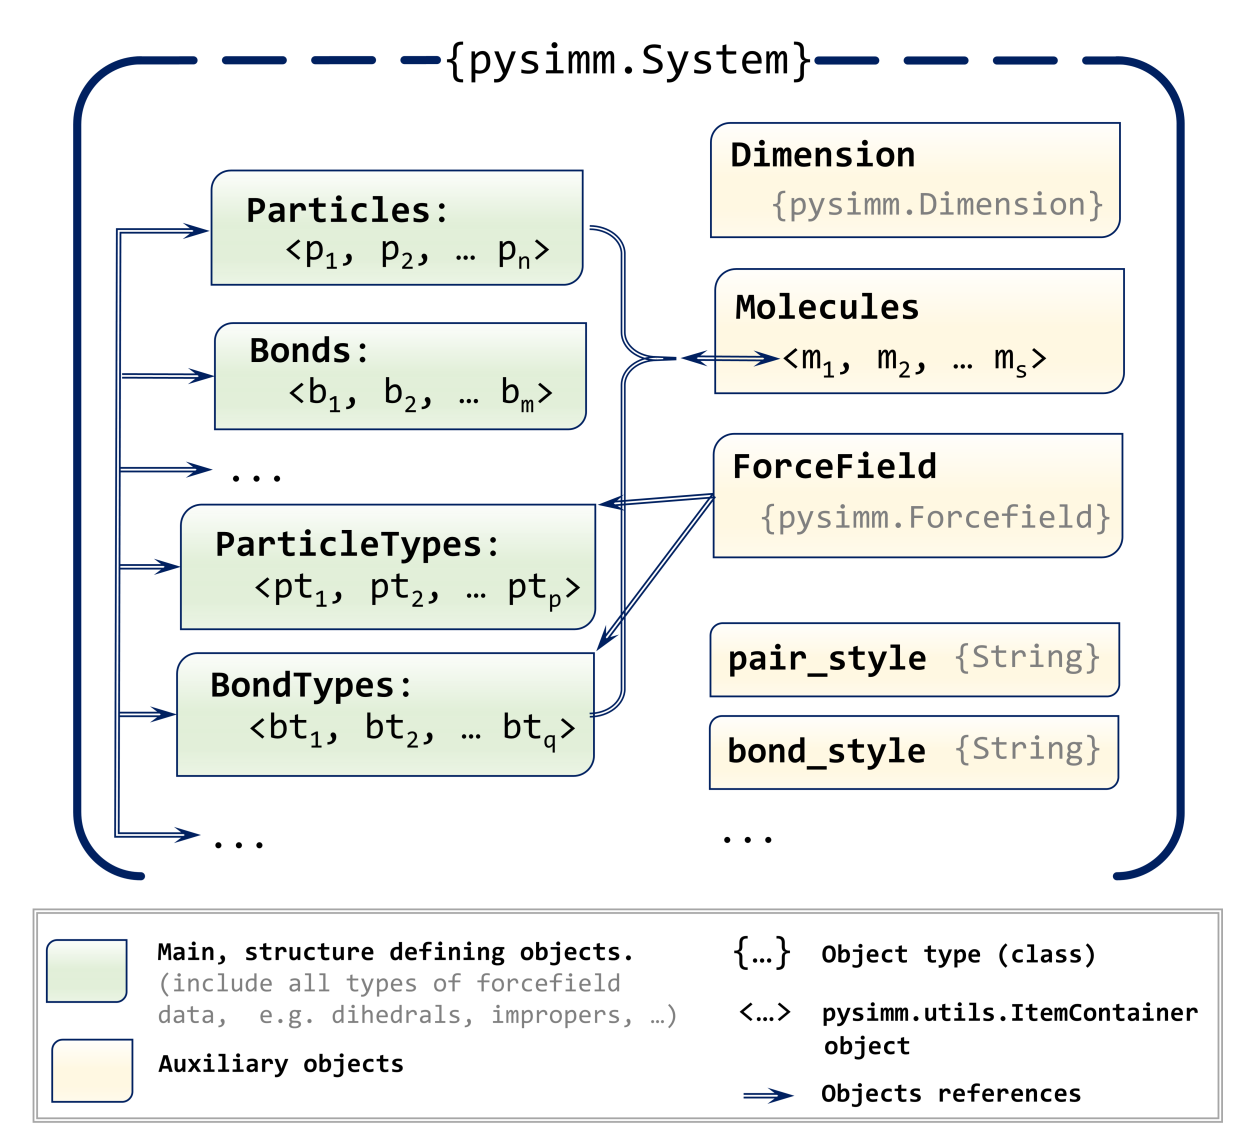
\includegraphics[width=0.95\columnwidth]{figures/figure1}
    \caption{Schematic representation of the \lstinline$system.System$ object that marks major fields of the object and their cross-references.}
    \label{sstm-scheme}
\end{figure}

Next, we need to add a molecule to our system. By default, our system \lstinline$s$ has a container object \lstinline$s.molecules$ that we need to add our new molecule to. We create a new molecule object, \lstinline$system.Molecule()$, and pass this to the molecule container class method \lstinline$s.molecules.add()$. This function returns the newly added object to the container, and we store this in variable \lstinline$m$.

\begin{lstlisting}
 m = s.molecules.add(system.Molecule())
\end{lstlisting}

Now that we have a place to contain all of our molecular data, we need to obtain data describing interactions between atoms from a force field. A \lstinline$forcefield.Forcefield$ object contains the parameters necessary to calculate the energy of your system as well as the logical typing rules for assigning the atom types to the particles of our system. In this example, we will use the GAFF2 force field and instantiate a \lstinline$Gaff2$ force field object that will be stored in variable \lstinline$f$:

\begin{lstlisting}
 f = forcefield.Gaff2()
\end{lstlisting}



This example assumes the user's knowledge on the GAFF2 atom types that are required for a methane molecule: i.e. "c3" and "hc". Let's get the \lstinline$system.ParticleType$ objects from our \lstinline$forcefield.Gaff2$ object that represent these atom types. Our \lstinline$forcefield.Gaff2$ object has a container object \lstinline$f.particle_types$ that organizes \lstinline$system.ParticleType$ objects and provides a method \lstinline$f.particle_types.get()$ to retrieve specific atom types based on names. The function returns a list of \lstinline$system.ParticleType$ objects, but in this example only one object is returned so we access the first element of the list. Instead of adding the \lstinline$system.ParticleType$ from f, we create a copy, and pass this newly created \lstinline$system.ParticleType$ object to a method that adds it to the particle type container object in our system \lstinline$s.particle_types$. The \lstinline$s.particle_types.add()$ method returns the newly added object, which we store as the GAFF2 atom type object representation.

\begin{lstlisting}
 gaff_c3 = s.particle_types.add( f.particle_types.get('c3')[0].copy())
 gaff_hc = s.particle_types.add( f.particle_types.get('hc')[0].copy())
\end{lstlisting}
Now we have a System object, \lstinline$s$, a Molecule object that is stored in our system, \lstinline$m$, and two GAFF2 atom type objects, \lstinline$gaff_c3$ and \lstinline$gaff_hc$. Let's start adding atoms.

First, we create the carbon atom (particle) at the origin. Initially, we will add the particle with zero charge, and will derive partial charges later. We instantiate a \lstinline$system.Particle$ object using keyword arguments to set the atom's coordinates x, y, z, the charge, the molecule this particle is a part of, and most importantly, the particle type, \lstinline$gaff_c3$. Notice that this is a reference to our \lstinline$system.ParticleType$ object that is in our \lstinline$system.System$ object, and not the \lstinline$forcefield.Gaff2$ object. Again we use a container add method to add our new particle to the particles container, and store the newly added particle in variable \lstinline$c1$.

\begin{lstlisting}
 c1 = s.particles.add(system.Particle( type=gaff_c3, x=0, y=0, z=0, charge=0, molecule=m))
\end{lstlisting}

The method \lstinline$add_particle_bonded_to$ of a \lstinline$system.System$ object allows the users to add a new particle that should be bonded to an existing particle in the system. If a force field object is also passed into this method, the new bonds, angles, and dihedrals will be created as necessary. The location of the new atom is selected randomly within a carbon-carbon bond length radius around the "parent" particle, and we will later use LAMMPS to perform structural optimization. For each hydrogen atom we want to add, we create a new \lstinline$system.Particle$ object, with zero charge and the \lstinline$gaff_hc$ type. We also need to identify this as a part of the molecule that already exists, m. This system.Particle object is passed to \lstinline$s.add_particle_bonded_to()$ as the first argument. The second argument is the particle that already exists in our system, in this case c1. The third argument is a reference to our \lstinline$forcefield.Gaff2$ object. The \lstinline$s.add_particle_bonded_to()$ method returns the newly added object, which we store as \lstinline$h1$, \lstinline$h2$, \lstinline$h3$ and \lstinline$h4$.

\begin{lstlisting}
 h1 = s.add_particle_bonded_to( system.Particle(type=gaff_hc, charge=0, molecule=m), c1, f)
 h2 = s.add_particle_bonded_to( system.Particle(type=gaff_hc, charge=0, molecule=m), c1, f)
 h3 = s.add_particle_bonded_to( system.Particle(type=gaff_hc, charge=0, molecule=m), c1, f)
 h4 = s.add_particle_bonded_to( system.Particle(type=gaff_hc, charge=0, molecule=m), c1, f)
\end{lstlisting}

Now we have added the particles to our system, but there is currently no simulation box. The \lstinline$system.System$ object has a method to construct a simulation box surrounding the atoms it contains, and optionally we can add padding around our molecule. Here we opt to use padding of 10 angstroms.

\begin{lstlisting}
 s.set_box(padding=10)
\end{lstlisting}
Before we optimize our structure, LAMMPS will need to know what type of pair, bond, and angle interactions we are using. These can be defined as string attributes of our \lstinline$system.System$ object.

\begin{lstlisting}
 s.pair_style='lj'
 s.bond_style='harmonic'
 s.angle_style='harmonic'
\end{lstlisting}

We will use the fire minimization algorithm implemented in LAMMPS. The \lstinline$lmps$ module in pysimm contains a series of shortcut methods to run some types of molecular mechanics simulation. In this case, we will use \lstinline$lmps.quick_min()$ to simultaneously setup and run the energy optimization of the system. The method requires the system object \lstinline$s$, and the minimization style \lstinline$min_style$ we want to use. Also, we will give each simulation a name so that all log files are kept in separate files.

\begin{lstlisting}
 lmps.quick_min(s, min_style='fire', name='fire_min')
\end{lstlisting}
More detailed discussion of the molecular mechanics simulation is in the next tutorial. The \lstinline$system.System$ class also has various methods to format our system data into different file types. Here we will output a PDB (protein data bank), and LAMMPS data file formats:
\begin{lstlisting}
 s.write_lammps('methane.lmps')
 s.write_pdb('methane.pdb')
\end{lstlisting}


\subsection{Tutorial II: Automatic force field assignment and MD simulations setup}

Construction of the whole system from scratch is clearly not the only option for creating the molecular mechanics simulation setup in pysimm. A much more common scenario is loading data from a text file to create the initial system (or several systems) which are then updated, modified, and merged using the API. Table \ref{tab:file_formats} lists text file formats common in computational chemistry that can be used to construct the \lstinline$system.System$ objects in pysimm. The files are read by the collection of static methods of \lstinline$system$ module which have name templates \lstinline$system.read_***$.     

Another utility that pysimm provides for convenient construction of small molecules is the interface to a PubChem database of compounds accessible through a RESTful API \cite{restful}. The interface allows users to create \lstinline$system.System$ objects from a PubChem SMILES query. In this example, we will use the SMILES string "CCO" to generate an ethanol molecule using the \lstinline$system.read_puchem_smiles()$ method. The function makes an HTTP request to the PubChem server, which returns an ASCII response formatted as a \textit{.mol} file. The text is interpreted as a \lstinline$system.System$ object that we store in variable ethanol. This system now contains elemental composition bond connectivity and bond orders.

\begin{lstlisting}
 ethanol = system.read_pubchem_smiles('CCO')
\end{lstlisting}
For this example to construct the model of the acetone molecule (the second specie of the mixture) let's use \lstinline$system.read_pdb()$ method to read the coordinates and topology information from the pdb-formatted text file and store the resulting \lstinline$system.System$ object in the variable with the corresponding name.

\begin{lstlisting}
 acetone = system.read_pdb('acetone.pdb')
\end{lstlisting}


\begin{table*}[bt!]
\caption{\label{tab:file_formats}File formats supported in pysimm to import data into \lstinline$system.System$ object}

\begin{tabular}{p{0.1\textwidth}p{0.2\textwidth}p{0.22\textwidth}p{0.38\textwidth}}
\toprule
Extension        & File format                      & Method name                                    & Notes        \\
\midrule
\textbf{json}    & ChemDoodle JSON                  & \lstinline$read_chemdoodle_json$          &               \\
\textbf{xyz}     & General XYZ record               & \lstinline$read_xyz$                      &               \\
\textbf{yaml}    & YAML serialisation of \lstinline$pysimm.system$ object    & \lstinline$read_yaml$                      &               \\
\textbf{lmps}    & LAMMPS input                 & \lstinline$read_lammps$            & Most developed and elaborate implementation. Allows among others to store FF information     \\
\textbf{cml}     & Chemical Markup Language file    & \lstinline$read_cml$           &      \\
\textbf{mol}     & MDL chemical table file          & \lstinline$read_mol$           &  Both 'V2000' and 'V3000' formats are supported \\
\textbf{pdb}     & Protein data bank file           & \lstinline$read_pdb$           &  Only particle position ('ATOM', 'HETATM') and bond ('CONECT') information is interpreted\\

\bottomrule
\end{tabular}
\medskip
\end{table*}

The next step is the application of the force field. We will need to use a FF object more than once, so we create a reference to it by instantiating the object and storing a reference to it in variable f.

\begin{lstlisting}
 f = forcefield.Gaff2()
\end{lstlisting}

Our \lstinline$system.System$ objects \lstinline$ethanol$ and \lstinline$acetone$ contain a class method \lstinline$apply_forcefield()$ that accepts a \lstinline$forcefield.Forcefield$ object and \textit{automatically} assigns force field parameters to systems. In this example we use our previously created \lstinline$forcefield.Gaff2$ object and pass it to the \lstinline$apply_forcefield()$ function, as well as specify we would like to derive Gasteiger charges \cite{gasteiger}.

\begin{lstlisting}
 ethanol.apply_forcefield(f, charges='gasteiger')
 acetone.apply_forcefield(f, charges='gasteiger')
\end{lstlisting}

Pysimm has a convenient method that inserts $N_k$ molecules of $k$ different types in a simulation box. The method is called \lstinline$system.replicate$, it requires a list containing the molecules and a list specifying the number of molecules of each type to insert. Additionally, it also takes density input in g/mL to set up the simulation box. Let's use it to make an initial box with 1-to-1 ethanol/acetone mixture.

\begin{lstlisting}
 s = system.replicate([ethanol, acetone], [200, 200], density=0.3)
\end{lstlisting}

Now that we have the initial system with molecules packed in a box, let's equilibrate it in 4 short steps. First, we carry out the energy minimization. Then we run 3 separate instances of molecular dynamics using the default 1 fs integration step for each: NVT MD for 10 ps at low density, and two NPT MD simulations for 100 ps each. At the beginning of the NVT simulation, we will generate new velocities at 100 K, and heat our system from 100 K to 300 K. At the beginning of the first NPT simulation, we will re-generate new initial velocities and start with a positive compressive pressure of 1000 atm which will be decreased to 1 atm during the run. Finally, the second NPT simulation will be held at 1 atm and 300 K to generate some sampling data. The settings for each of those simulation steps are configured as a simple Python dictionary where keys closely follow the names of corresponding commands in LAMMPS. The settings use LAMMPS "real" system of units (time in fs, distance in $\AA$, energy in Kcal/mole, see the LAMMPS documentation \cite{lmps:units}), and have default values defined for each keyword (see the pysimm documentation).

\begin{lstlisting}
 min_settings = {'name': 'fire_min', 'min_style': 'fire'}
\end{lstlisting}

\begin{lstlisting}
 nvt_settings = {'name': 'nvt_md', 'ensemble': 'nvt',
    't_start': 100, 't_stop': 300, 'new_v': True,
     'length': 10000, 'timestep': 1}
\end{lstlisting}

\begin{lstlisting}
 npt1_settings = {'name': 'npt_md', 'ensemble': 'npt',
    'temp': 300, 'new_v': True,
    'p_start': 1000, 'p_stop': 1,
    'length': 100000, 'timestep': 1}
\end{lstlisting}

\begin{lstlisting}
 npt2_settings = npt1_settings.copy()
 npt2_settings['p_start'] = 1
\end{lstlisting}

Let's instantiate the LAMMPS simulation object that governs the simulation process and will contain other setting objects responsible for various aspects of the simulation. Right away let's add to the simulation container the \lstinline$OutputSettings$ object which will define the style and print frequency of LAMMPS simulation output. 

\begin{lstlisting}
 sim = lmps.Simulation(s)
 sim.add(lmps.OutputSettings( thermo={'freq': 500, 'style': 'custom', 
'args': ['step', 'temp', 'etotal', 'press', 'density']}))
\end{lstlisting}

Next, we add an optimization object and a molecular dynamics object using corresponding methods of the \lstinline$lmps.simulation$ -- they will be added to the LAMMPS script (and thus executed) in the order they appear in the code. Finally, we send the \lstinline$run$ command that starts the whole simulation sequence.

\begin{lstlisting}
 sim.add_min(**min_settings)
 sim.add_md(**nvt_settings)
 sim.add_md(**npt1_settings)
 sim.add_md(**npt2_settings)
 sim.run()
\end{lstlisting}

In the present setup it is easy to replace the GAFF-2 force field with a different one (one of the supported by the API). To use a different FF one changes the reference to the FF object: write \lstinline$f = forcefield.Charmm()$ instead of \lstinline$f = forcefield.Gaff2()$, and re-run the above workflow.

In the final part of this tutorial let's see how the same equilibration simulations will differ if molecules are typed with a different FF. As an example let's use CHARMM general force field (CGenFF). Similar to GAFF, pysimm can automatically recognize and type most common CGenFF atom types for H, C, N, O, and S chemical elements.

After the simulations are finished we can parse the output log file and draw the density of the system during the overall 200 ps of both NPT runs. Figure \ref{ff-diff} shows the density of acetone-ethanol 1-to-1 mixture as read from the LAMMPS logs of 2 similar NPT simulations that use GAFF2 and CGenFF force fields. The results are close to each other and in this case the difference is likely caused by the difference in compatibility of corresponding FF with Gasteiger partial charges. 

\begin{figure}[htbp]
  \centering
    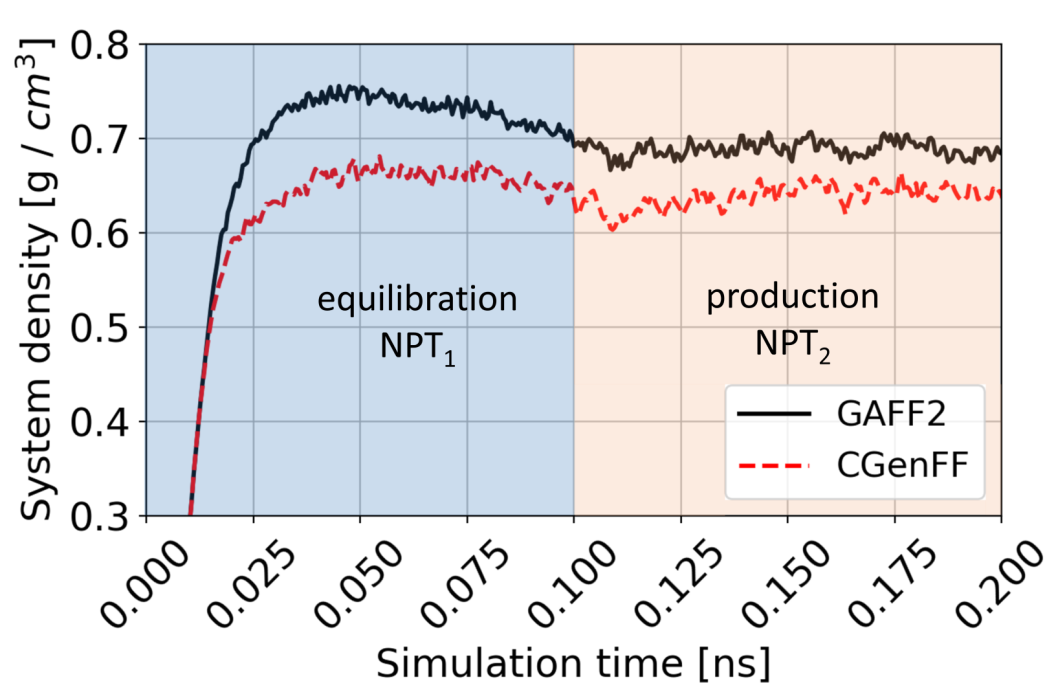
\includegraphics[width=0.9\columnwidth]{figures/figure5}
    \caption{Comparison of ethanol/acetone 1-to-1 mixture density simulated with the usage of GAFF2 and CGenFF forcefields. The LAMMPS simulation setup and automatic FF typing are done in pysimm}
    \label{ff-diff}
\end{figure}

\subsection{Tutorial III: Simulated random walk polymerization with pysimm}

\subsubsection{Preparing the repetitive unit}

Let's load the repetitive unit of the polymer creating \lstinline$system.System$ object from a .pdb file that has \lstinline$'CONECT'$ information (pysimm can interpret this data to make bonds between the atoms of the system). The \lstinline$system.read_pdb$ method supports additional string parameter that points to the CHARMM stream (.str) file which can be used to update the charges of the particles in the system.

\begin{lstlisting}
sst = system.read_pdb( '../data/cbma_monomer.pdb', str_file='../data/cbma_monomer.str')
\end{lstlisting}

To display the repetitive unit on the Jupyter canvas, let's use nglview package. It also can show additional label information for each atom; e.g. indexes of all atoms of the system. Alternatively, if nglview is not available, we encourage the user to open the imported structure in any other standalone molecular viewer (like VMD \cite{vmd} or Avogadro \cite{avogadro}). 

\begin{lstlisting}
view = nglview.show_structure_file( '../data/cbma_monomer.pdb')
view.add_label(color='black', scale=1.3, labelType='text', zOffset=2.0, attachment='middle_center', labelText = [str(pt.tag) for pt in sst.particles])
\end{lstlisting}


Figure \ref{rep-unit} shows an example of the definition of the head and tail atoms in the carboxybetaine methacrylate [CBMA] repetitive unit. As shown above, the undercoordinated carbon atoms (carbons with incomplete valency) have indices 1 and 2. They will be the head (the atom with which the current repeating unit connects to the previous repeating unit) and the tail (the atom to which the next repeating unit connects) during the pysimm polymerization process. Let's mark those atoms with the corresponding text labels in our system

\begin{lstlisting}
lnkr_atoms = {'head': 1, 'tail': 2}
for k, v in lnkr_atoms.items():
    sst.particles[v].linker = k
\end{lstlisting}

\begin{figure}[htbp]
  \centering
    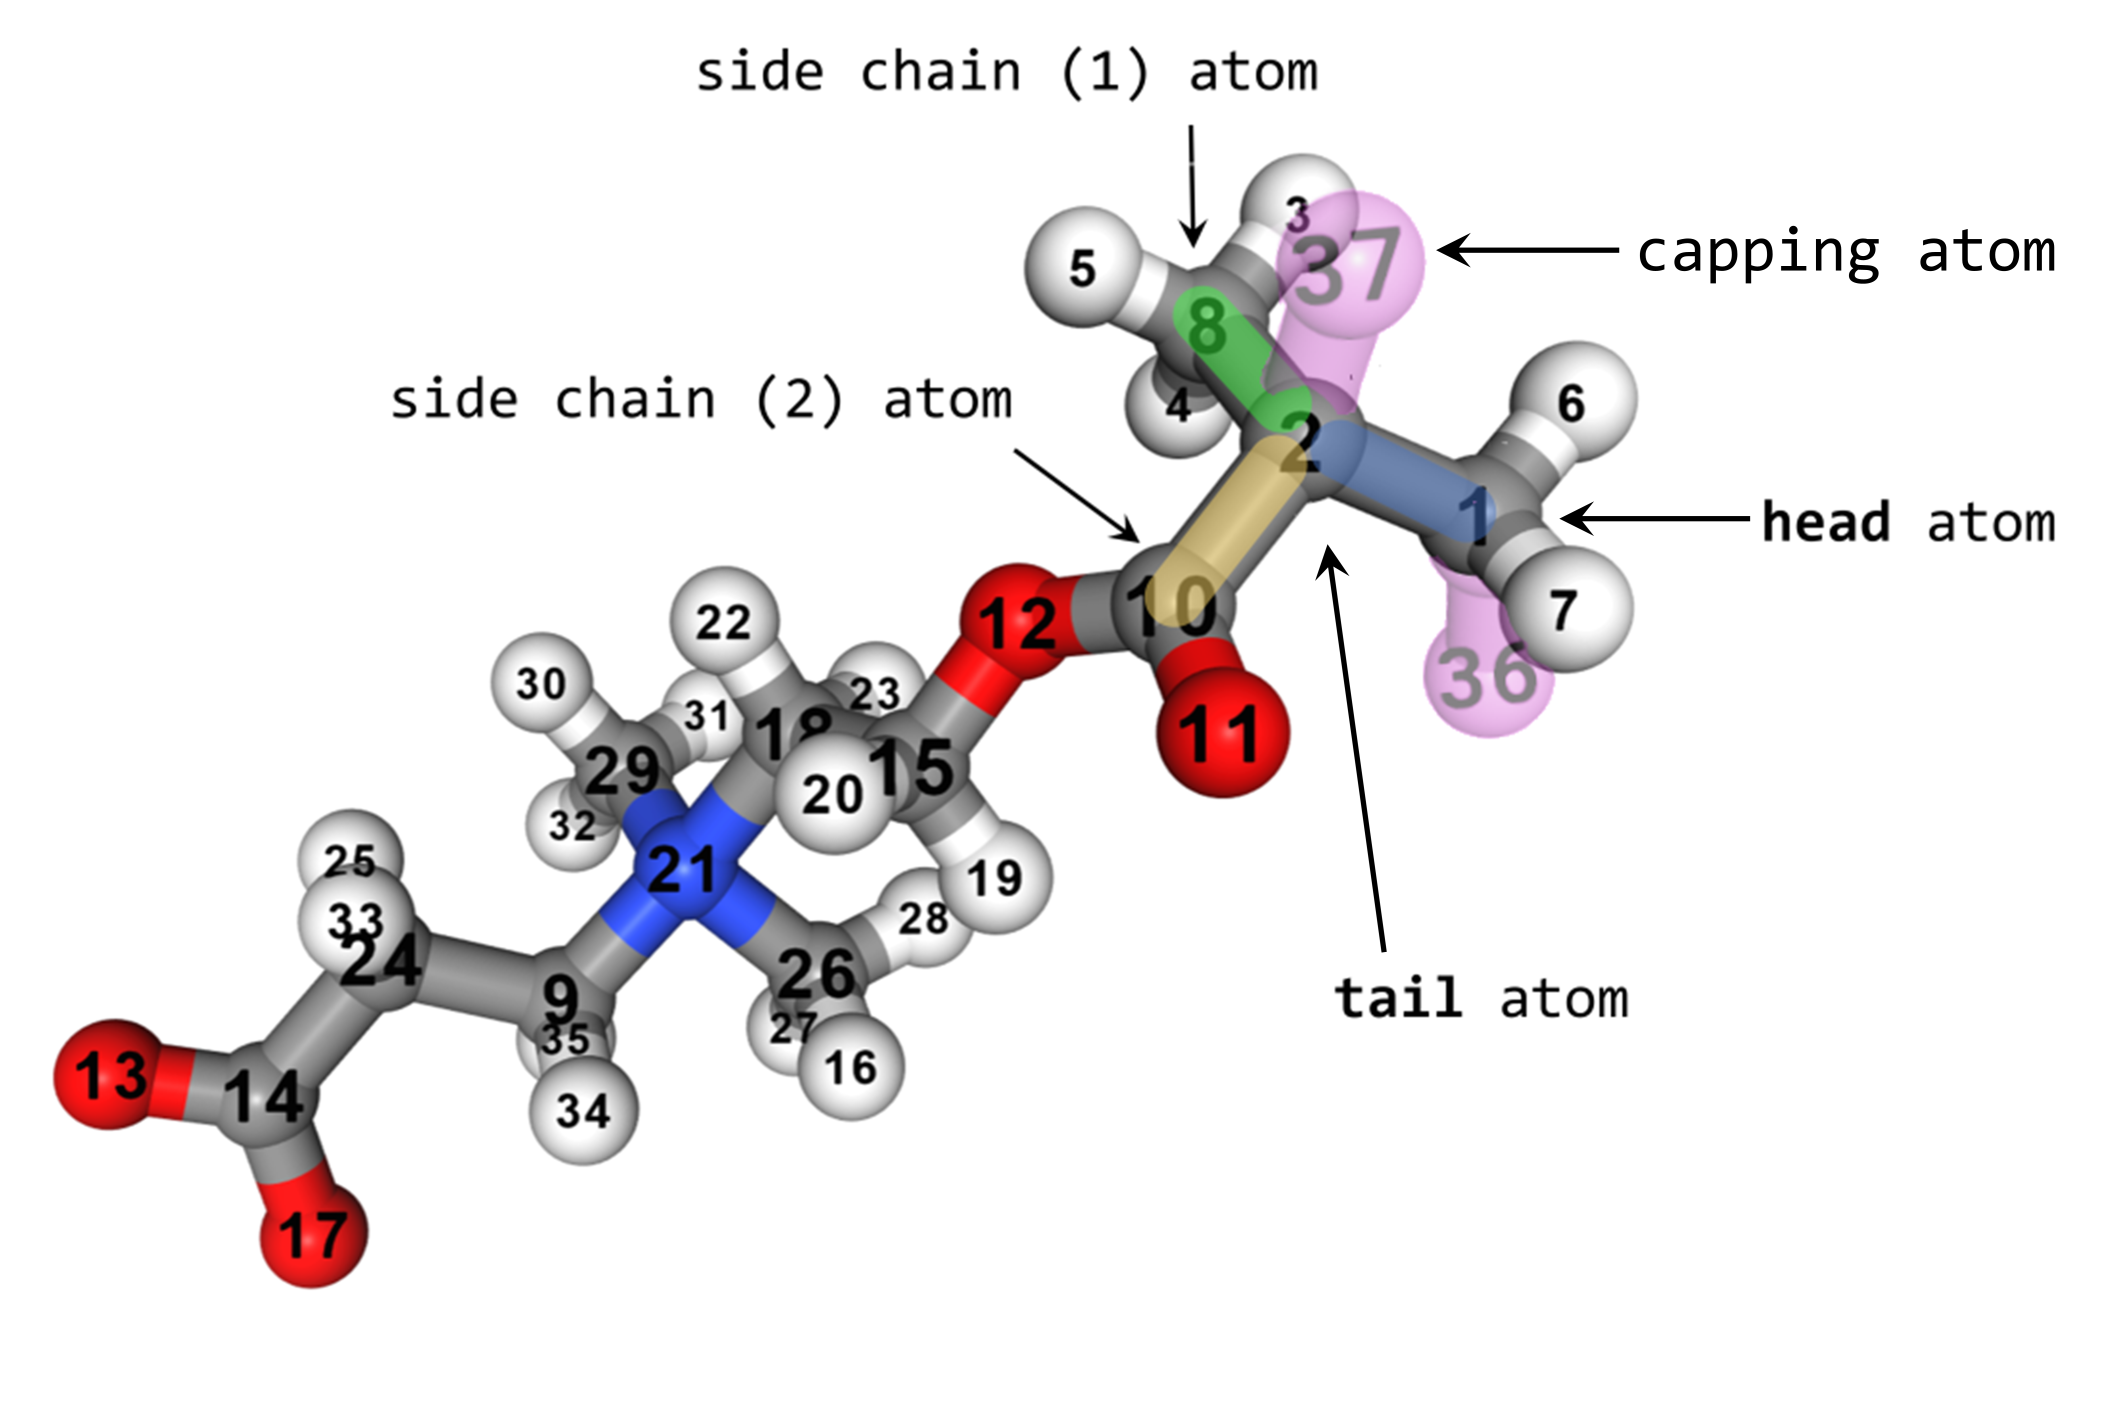
\includegraphics[width=0.9\columnwidth]{figures/figure2_mod}
    \caption{Detailed description of the atoms in the CBMA repetitive unit, that is important for the polymerization and the tacticity analyzer methods of \lstinline$pysimm.random_walk$}
    \label{rep-unit}
\end{figure}

Let's type the repetitive unit with the basic pysimm CGenFF automatic typing tool. The charges of all particles were read from the .str file, so there is no need to reassign them (if not, pysimm can do it using e.g. the Gasteiger method)

\begin{lstlisting}
ff = forcefield.Charmm()
sst.apply_forcefield(ff, charges=None)
\end{lstlisting}


\subsubsection{Making the polymer and checking its tacticity}

Once the FF types and charges are defined, one can use the force field assisted random walk method. The method requires the \lstinline$system.System$ object representing a monomer, and the integer number of monomers to be concatenated.  The other optional (keyword) arguments presented in the example define the density of the final output system, flag to indicate to output the construction trajectory (in .xyz format), and a flag to indicate whether the final chain will be unwrapped. Let's build a short (15 repetitive units) chain.

\begin{lstlisting}
sngl_chain = random_walk(sst, 15, forcefield=ff, density=0.01, traj=False, unwrap=True)
\end{lstlisting}

Next, let's check the tacticity of the created oligomer. The \lstinline$check_tacticity()$ method of the \lstinline$random_walk$ application analyzes the local geometry of atoms for polymers that can have tacticity. The method returns the distribution of meso-to-racemo diads along the backbone of the macromolecule (as shown in Figure \ref{diads:scheme}).

\begin{figure}[htbp]
  \centering
    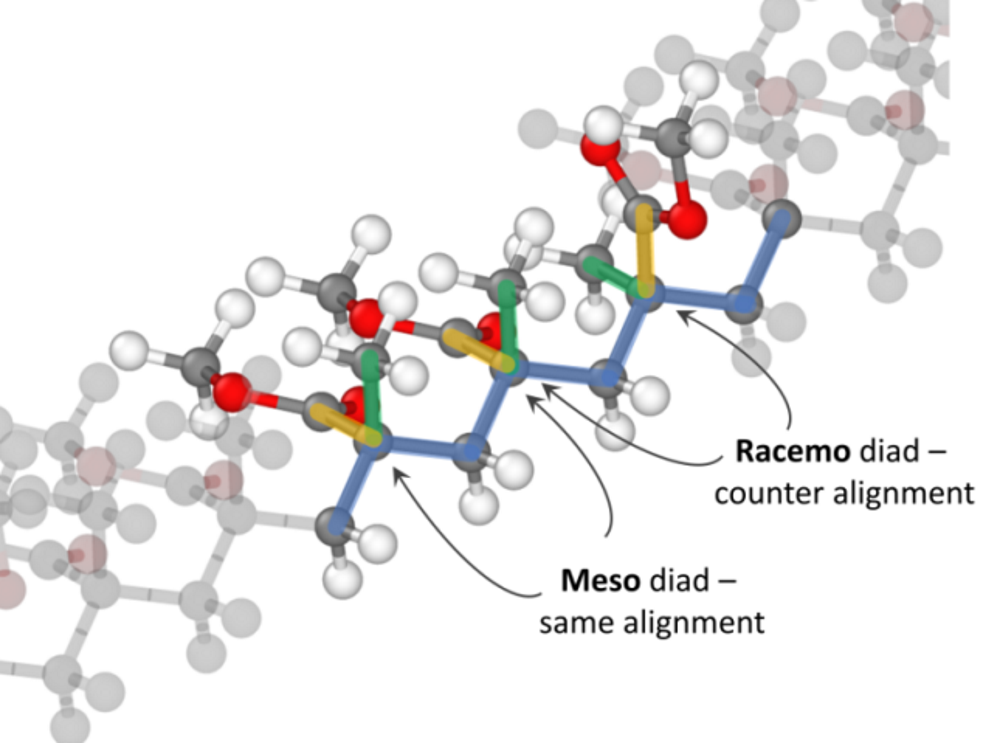
\includegraphics[width=0.85\columnwidth]{figures/figure3}
    \caption{Schematic representation of a meso and a racemo diad along the polymer backbone. In the case of a meso diad both the blue-green-yellow vector triples of the two consecutive monomers have the same alignment, whereas in a racemo diad, one of the blue-green-yellow vector triples is right-handed while the other is left-handed.}
    \label{diads:scheme}
\end{figure}

The input parameters for the method are:
\begin{itemize}
 \item A pysimm system that represents a macromolecule.
 \item A list with 4 integers that defines the indices of the node atoms in a repetitive unit of the macromolecule. The indices in their order represent: (1) the first atom of the backbone; (2) the second atom of the backbone; (3) the first atom of the first side chain (or methyl, or hydrogen); (4) the first atom of the second side chain. Note that the colors of the atom indices match the colors of the vectors on the figure \ref{diads:scheme}. 
 \item Number of atoms (particles) in the repetitive unit of the macromolecule
\end{itemize}

The second variable of the \lstinline$check_tacticity$ output is the list that shows whether each two consecutive repetitive units in the chain form either a meso (True) or a racemo (False) diad. Let's examine the obtained chain and print the result in the form of a simple 2-column histogram that shows the number of meso and racemo diads in the chain. The indices for the analyzed repetitive unit are highlighted in figure \ref{rep-unit}, and they are 1, 2, 8, and 10.

\begin{lstlisting}
tacticity_stat = check_tacticity(sngl_chain, [1, 2, 8, 10], len(sst.particles))
\end{lstlisting}

In this case, among 15 monomers (thus 14 diads), we see that most diads have a meso configuration (figure \ref{diads:distr}-(a)), meaning that the majority of the monomer pairs in the chain have the same orientation. Only a very few monomer pairs (10\%-30\%, depending on the run) will form racemo diads. In this implementation of the random walk there is no explicit control of the following monomer orientation, hence all monomers attached initially had to form meso diads. However, due to the geometry optimization and short MD simulations that are implemented in the random walk method, the orientation of neighboring monomers occasionally can switch, thus giving some number of racemo diads. Therefore, depending on the strength of the energy barrier for rotation, during longer MD simulations the polymer can relax to an atactic state. However, pysimm can also allow gaining more control over the polymer tacticity.


\subsubsection{Polymerization with controlled tacticity}
While polymers synthesized through conventional radical polymerization are usually atactic, newer polymerization catalysts are able to offer high purity syndiotactic or isotactic polymers, often with markedly different physical properties. In this part, let's concentrate on building models of syndiotactic or isotactic polymers. We will use another method which is called \lstinline$random_walk_tacticity$, which allows the user to define the orientation of the next attached monomer during the polymer building phase. For that, some additional modifications should be done to the repetitive unit that was previously used. The \lstinline$random_walk_tacticity$ method requires a capped monomer, therefore let's add capping carbon atoms to the linker atoms of our repetitive unit (atoms with tags 1 and 2, see figure \ref{rep-unit}). The capping atoms (ones with tags 36 and 37 on figure \ref{rep-unit}) are dummy atoms, so we can assign them any types, for convenience, let's reuse a type that is already present in our system: like \lstinline$'CG321'$ an $sp^3$ hybridized carbon with 2 hydrogen atoms attached. Moreover, the capping atoms will be undercoordinated, but it is not important in this case, as they are dummy atoms and will be removed during the simulated polymerization.

Both capping atoms should be decorated with an additional field named \lstinline$rnd_wlk_tag$ that contains a string with either \lstinline$'head_cap'$ or \lstinline$'tail_cap'$ value, respectively. Finally, another label \lstinline$linker='mirror'$ should be assigned to an atom of the system; the atom with this label together with 2 labeled atoms of the backbone will be used to build a mirror plane for construction of the reflected repetitive unit for syndiotactic insertion. In our case, the most convenient \lstinline$'mirror'$ atom is the freshly added \lstinline$'head_cap'$ atom (it will be connected to the atom \#1 to the vacant position of the tetrahedron formed by atoms with tags 2, 6, and 7; see figure \ref{rep-unit}).

To shorten the tutorial text we do not list the whole code that performs the aforementioned labeling, but only the first and last lines of it (please refer to the code in \textit{.py} or \textit{.ipynb} files for the implementation with detailed inline commentaries).

\begin{lstlisting}
new_sst = sst.copy()
captype = new_sst.particle_types.get( 'CG321')[0]
...
new_sst.objectify()
\end{lstlisting}

Note that preparations written above are not needed if capping atoms are already present in the initial structure of the repetitive unit. Please, refer to example 12 of pysimm distribution, where the tacticity-controlled polystyrene chain is built  (\textit{Examples/12\_tacticities/polystyrene\_nosim.py}).

To control the tacticity of the chain, the method has \lstinline$tacticity$ keyword argument that accepts a real number $n \in [0,\ 1]$, which defines the relative number of isotactic insertions (note that generally for any value $n \in (0, 1)$ the polymer is considered atactic). Thus, $n = 1$ will be a fully isotactic chain, $n = 0$ will be syndiotactic chain, whereas $n = 0.5$ will be a chain with equal number of isotactic and syndiotactic insertions. This method also accepts keyword strings as values of tacticity key. One can use either $n = 1$ or 'isotactic', $n = 0$ or 'syndiotactic', and $n = 0.5$ or 'atactic'. For more details and options of \lstinline$random_walk_tacticity$ method please refer the pysimm documentation.

First, let's run the \lstinline$random_walk_tacticity$ in "no simulation" mode. In that regime next monomer will be put to an approximately correct, geometrically calculated position without the FF optimization and NVE molecular dynamics simulations.

\begin{lstlisting}
polymer_nosim = random_walk_tacticity(new_sst, 15, forcefield=ff, sim='no', tacticity='syndiotactic', density=0.01)
\end{lstlisting}

The result is a syndiotactic chain, and all diads in this case are clearly racemo- diads (figure \ref{diads:distr}-(b)). Now let's do the same but with FF optimization of the growing polymer chain between every monomer insertion, and see how many diads will be reconfigured from racemo- to meso- geometry.

\begin{lstlisting}
polymer = random_walk_tacticity(new_sst, 15, forcefield=ff, tacticity=0.0)
\end{lstlisting}

The figure \ref{diads:distr}-(c) confirms that the optimization can change the initial distribution of the monomer orientations. However, the chain obtained with \lstinline$random_walk_tacticity$ has more racemo than meso diads (as the example was based on creating a syndiotactic polymer), compared to the chain obtained by the original \lstinline$random_walk$ method (10\%-30\%).

\begin{figure}[htbp]
  \centering
    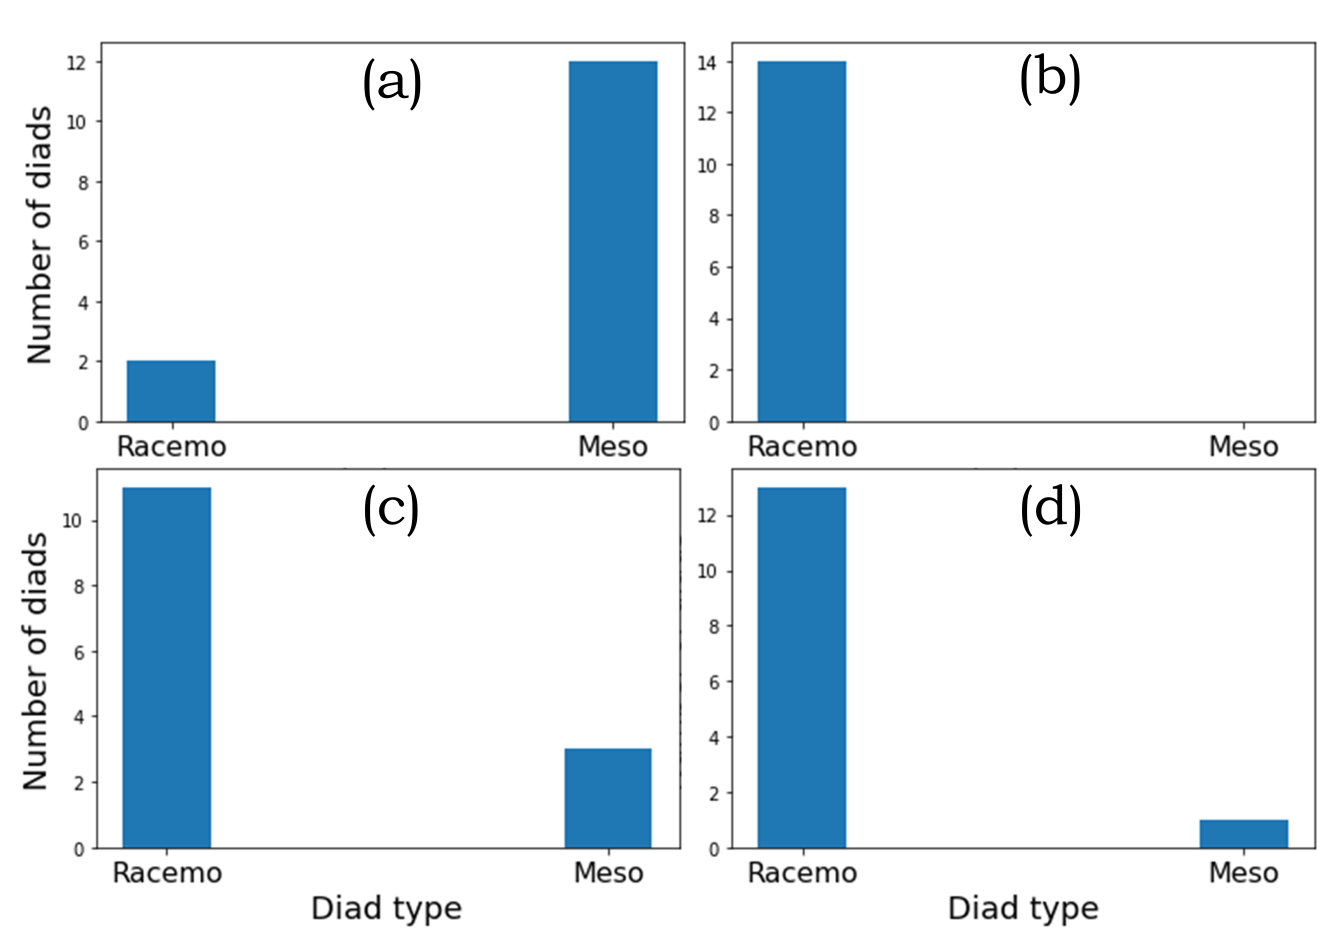
\includegraphics[width=0.95\columnwidth]{figures/figure4}
    \caption{Meso-to-racemo diad distribution in a single pCBMA chain containing 15 repetitive units made with different methods of \lstinline$pysimm.random_walk$ application. (a) Standard \lstinline$random_walk$ method. (b) \lstinline$random_walk_tacticity$ method with no simulations applied, (c) \lstinline$random_walk_tacticity$ method with simulations on, (d) \lstinline$random_walk_tacticity$ run with a post-optimization.}
    \label{diads:distr}
\end{figure}

\subsubsection{A setup to construct a polymer chain with exact tacticity}

In the previous section it was shown that in pysimm, one can easily construct a "no-simulation" polymer chain. The simple chain (but illustrative for tacticity explanations) is constructed by connecting the repetitive units to each other without force field simulations. The tacticity of that chain is easy to set to be exact, unlike the tacticity of a chain built with the FF simulations enabled.

The robustness of the FF functional form allows one to run the simulations using the polymer chain built by \lstinline$random_walk_tacticity$ with \lstinline$no_sim$ flag on as an initial structure. Long enough MD simulation with the fixed (via SHAKE) angles between the side chains will result in a relaxed polymer chain with exactly the same tacticity as it was constructed at the beginning. Please note, that depending on the geometry of your repetitive unit, the initial structure of the chain of concatenated repetitive units might be defined approximately. If possible we recommend putting the linker atoms (head and tail atoms) into anti-periplanar positions (see the CBMA repetitive unit in this tutorial, figure \ref{rep-unit}).

Below is a small code sample that sets up (in pysimm) the MD simulations using the 'no simulation' configuration and results in a relaxed polymer chain. First let's invoke the \lstinline$Simulation$ object of the \lstinline$pysimm.lmps$ module using the copy of the initial "no simulation" polymer chain.
\begin{lstlisting}
pmer_shake = polymer_nosim.copy()
sim = lmps.Simulation(pmer_shake, name='shake_relax', log='shake.log')
\end{lstlisting}

Next, let's add a SHAKE directive to the simulation. The aim is to keep the angle between the side chains of each repetitive unit fixed (figure \ref{rep-unit}). To apply shake to an angle in LAMMPS, the user is required to know the identifiers of bond types for the corresponding angle and the identifier of the angle type. Presume here, that we don't know the indexes of corresponding bonds and angle, but we know the types of particles that form this angle, which will give us the required indexes. 
\begin{lstlisting}
bnd1 = polymer.bond_types.get( 'CG2O2,CG301')[0].tag
bnd2 = polymer.bond_types.get( 'CG301,CG331')[0].tag
angl = polymer.angle_types.get( 'CG331,CG301,CG2O2')[0].tag
sim.add_custom('fix shck_fix all shake 0.001 40 0 b {} {} a {}'.format(bnd1, bnd2, angl)
\end{lstlisting}
Finally, let's run a short (30 ps) NVE MD simulation with a single built chain to give it enough time to relax all non-fixed bonds, angles and dihedrals.
\begin{lstlisting}
sim.add_md(ensemble='nve', limit=0.1, length=30000)
sim.run()
pmer_shake.unwrap()
\end{lstlisting}

The tacticity of the resulting chain remains almost perfectly syndiotactic, as it was before the relaxing MD simulation (figure \ref{diads:distr} (b) and (d)). The exception is the geometry of the terminal repetitive unit that eventually can switch during the MD run, giving one meso diad.



\section{Author Contributions}
%%%%%%%%%%%%%%%%
% This section must describe the actual contributions of
% author. Since this is an electronic-only journal, there is
% no length limit when you describe the authors' contributions,
% so we recommend describing what they actually did rather than
% simply categorizing them in a small number of
% predefined roles as might be done in other journals.
%
% See the policies ``Policies on Authorship'' section of https://livecoms.github.io
% for more information on deciding on authorship and author order.
%%%%%%%%%%%%%%%%

AGD, BLAP, MEF and CMC conceived and wrote the online tutorials 1 and 2. All authors conceived and wrote tutorial 3 and contributed to manuscript writing. AGD maintains the source repository of the project at GitHub.

% We suggest you preserve this comment:
For a more detailed description of author contributions,
see the GitHub issue tracking and changelog at \githubrepository.

\section{Other Contributions}
%%%%%%%%%%%%%%%
% You should include all people who have filed issues that were
% accepted into the paper, or that upon discussion altered what was in the paper.
% Multiple significant contributions might mean that the contributor
% should be moved to authorship at the discretion of the a
%
% See the policies ``Policies on Authorship'' section of https://livecoms.github.io for
% more information on deciding on authorship and author order.
%%%%%%%%%%%%%%%

The authors would like to acknowledge other pysimm developers and testers: Ping Lin, Dylan Anstine, Grit Kupgan, Shalini Jayaraman Rukmani, and Aravinda Munasinghe. 

% We suggest you preserve this comment:
For a more detailed description of contributions from the community and others, see the GitHub issue tracking and changelog at \githubrepository.

\section{Potentially Conflicting Interests}
%%%%%%%
%Declare any potentially competing interests, financial or otherwise
%%%%%%%

The authors declare no potential conflict of interests.

\section{Funding Information}
%%%%%%%
% Authors should acknowledge funding sources here. Reference specific grants.
%%%%%%%
The authors would like to acknowledge U.S. Department of Energy for funding (grant DE-FG02-17ER16362).

\section*{Author Information}
\makeorcid

\bibliography{references}

%%%%%%%%%%%%%%%%%%%%%%%%%%%%%%%%%%%%%%%%%%%%%%%%%%%%%%%%%%%%
%%% APPENDICES
%%%%%%%%%%%%%%%%%%%%%%%%%%%%%%%%%%%%%%%%%%%%%%%%%%%%%%%%%%%%

%\appendix


\end{document}